\subsubsection*{Motoren}
\addcontentsline{toc}{subsubsection}{Motoren}


Nach den Berechnungen in Abbildung \ref{fig:Auslegung_Antrieb}  wurden zwei passende Motoren ausgewählt, bestellt und anschliessend getestet. Entscheidende Faktoren bei der Auswahl waren das Drehmoment und die Betriebsspannung. Die Drehzahl des ausgewählten Motors ist tiefer als die anfangs vorgesehene Drehzahl. Dadurch ist die maximale Geschwindigkeit des Roboters tiefer als gewünscht. Dies wird für den Prototyp jedoch in kauf genommen. Die Befestigung der Motoren an dem gebauten Fahrwerk Prototyp sind auf Abbildung \ref{fig:Motorenaufbau} ersichtlich.

\begin{figure}[H]
    \centering
    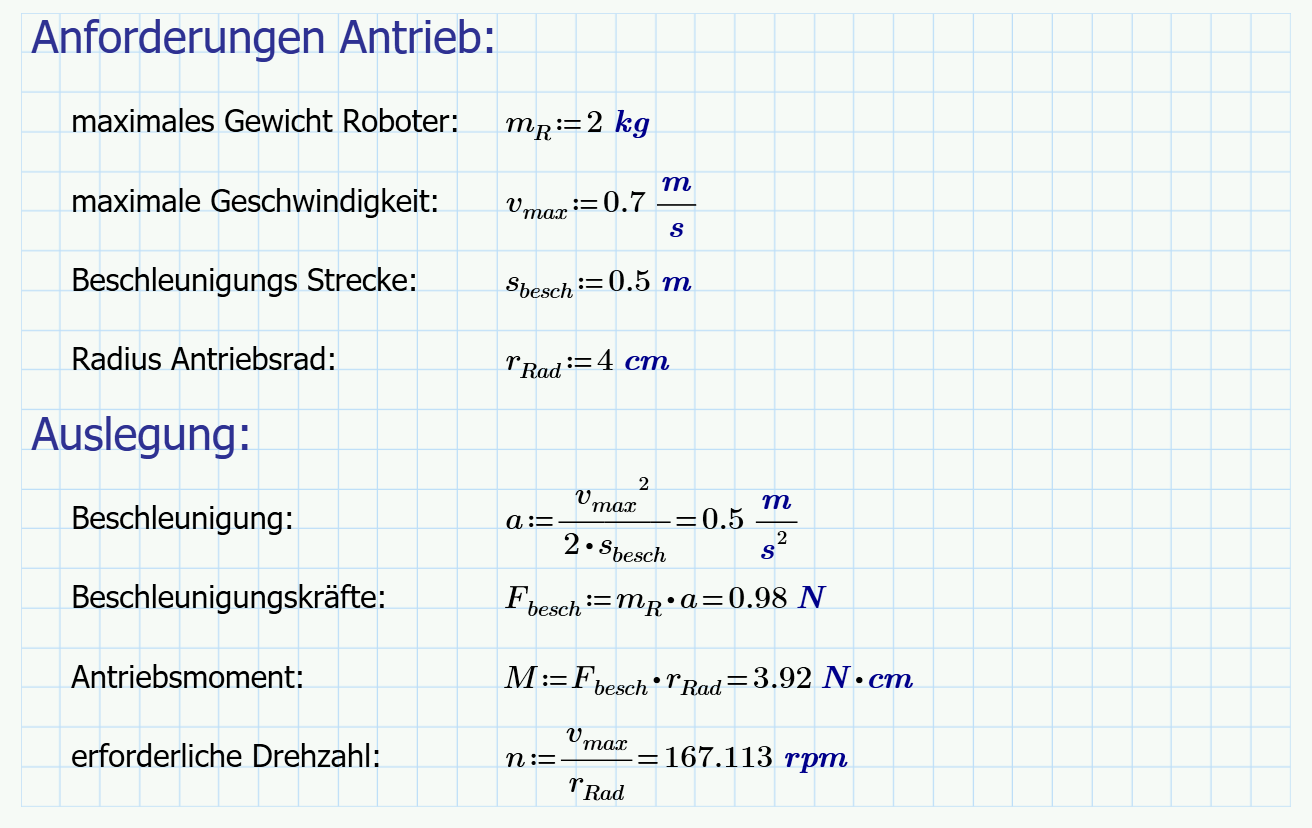
\includegraphics[width=0.8\linewidth]{img/Auslegung_Antrieb.PNG}
    \caption{Auslegung Antrieb}
    \label{fig:Auslegung_Antrieb}
\end{figure}

\begin{figure}[H]
    \centering
    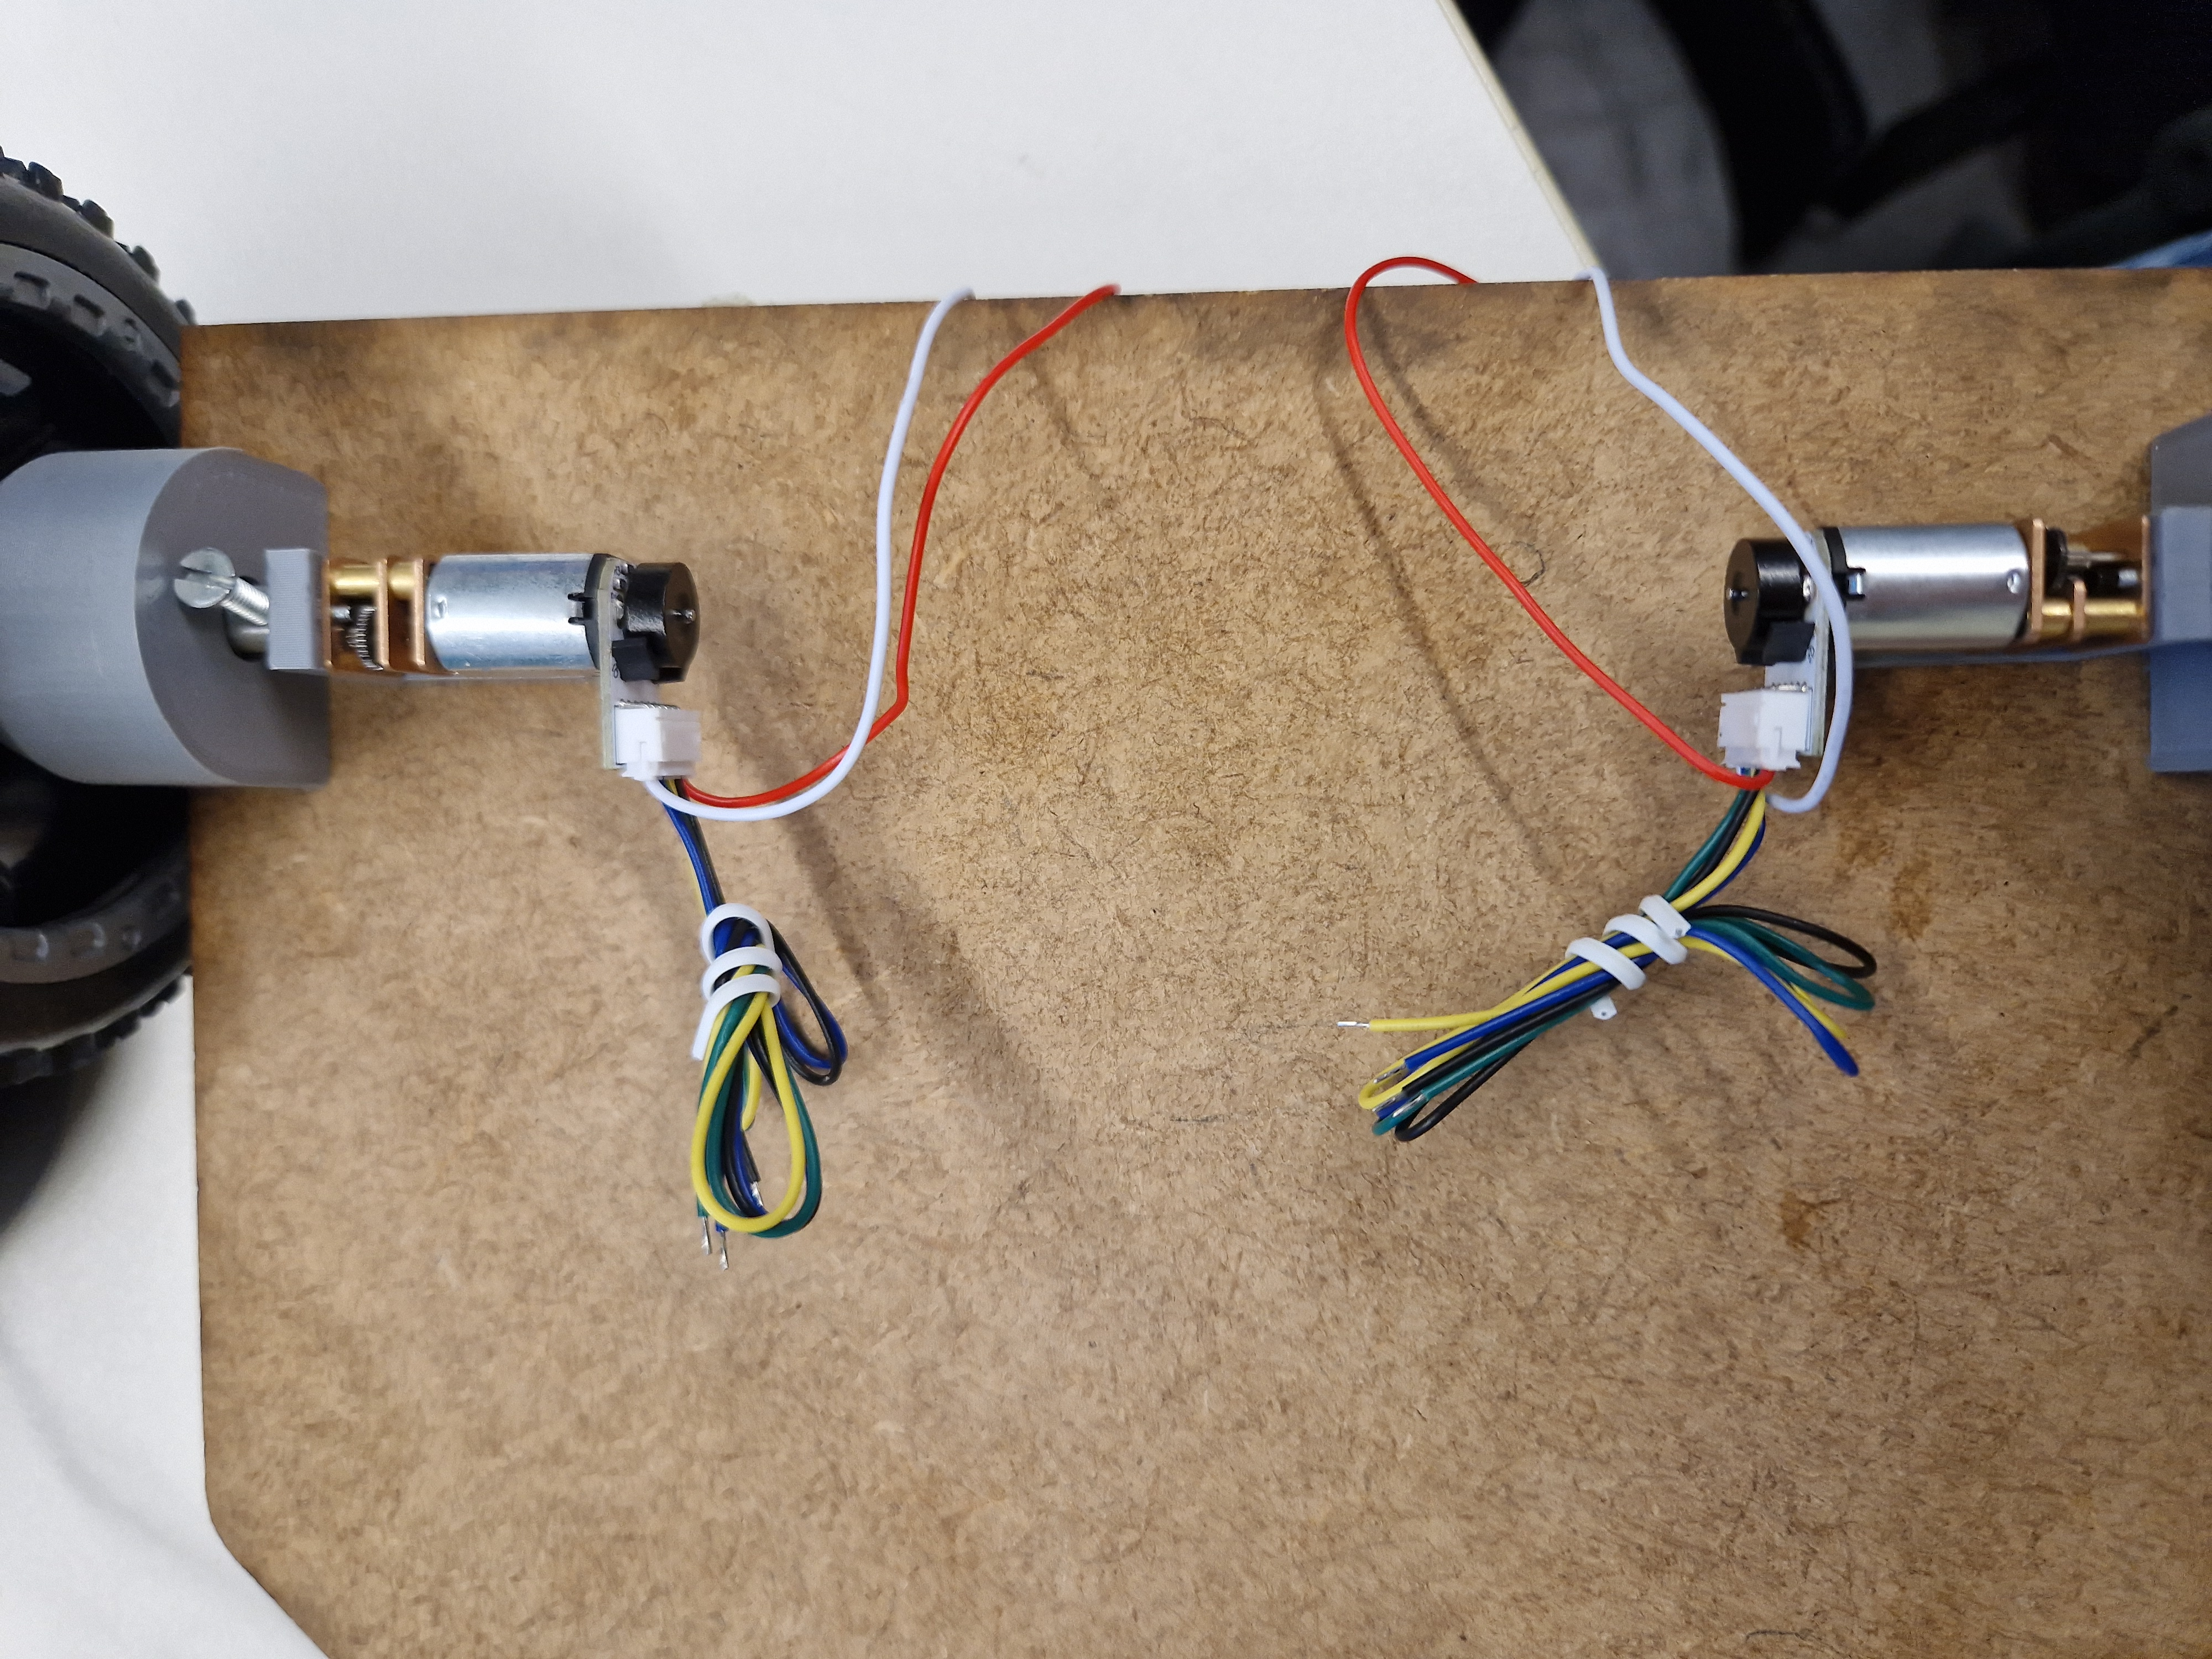
\includegraphics[width=0.8\linewidth]{img/Motorenaufbau.jpg}
    \caption{Motorenbefestigung Prototyp}
    \label{fig:Motorenaufbau}
\end{figure}

Der Test bestand darin, den Motor mit einer \acrfull{pwm} bei zwei unterschiedlichen Spannungen zu betreiben. Zunächst wurde der Motor mit einer Spannung von 5V getestet. Dabei wurde der \gls{duty-cycle} schrittweise erhöht, bis der Motor bei 58\% des \gls{duty-cycle}s zu drehen begann. Nachdem der Motor gestartet war, konnte der \gls{duty-cycle} auf bis zu 44\% reduziert werden, bevor der Motor wieder stoppte.

In einer zweiten Testsequenz wurde die gleiche Vorgehensweise mit einer Spannung von 12V durchgeführt. Hier begann der Motor bei einem \gls{duty-cycle} von 33\% zu drehen. Beim schrittweisen Reduzieren der Einschaltzeit, drehte der Motor bis zu einem \gls{duty-cycle} von 12\% weiter.

Da der Motor möglichst präzise gesteuert werden soll, ist eine feine Einstellung der Drehzahl erforderlich. Der Test zeigte jedoch, dass der Motor bei 5V nur verzögert anlief, was zu einer zu schnellen Drehbewegung führen könnte und die präzise Steuerung erschwert. Streuverluste sowie die Bauart des Motors erfordern einen höheren Anlaufstrom.

Um dennoch eine geringe Anfangsdrehzahl zu gewährleisten, wird der Motor initial mit 12V gestartet. Sobald der Motor angelaufen ist, wird die Spannung auf 5V reduziert, wodurch der Motor bei hohen \gls{duty-cycle} nicht überlastet wird. Die Ergebnisse der Spannungstest sind in Tabelle \ref{tab:dutycycle} ersichtlich.

\begin{table}[H]
\centering
\begin{tabularx}{\textwidth}{|c|>{\centering\arraybackslash}X|>{\centering\arraybackslash}X|}
\hline
\textbf{Spannung} & \textbf{Einschaltzeit (Duty Cycle)} & \textbf{Ausschaltzeit (Duty Cycle)} \\ \hline
12V & 33\% & 12\% \\ \hline
5V  & 58\% & 44\% \\ \hline
\end{tabularx}
\caption{Vergleich der Duty-Cycle-Werte bei 12V und 5V}
\label{tab:dutycycle}
\end{table}

\subsubsection*{Tiny K22 Pinout} \label{Blockdiagramm: Schnittstellen zwischen den Komponenten}
\addcontentsline{toc}{subsubsection}{Tiny K22 Pinout}

Für die hardwarenahe Steuerung und Regelung wurde ein \gls{tinyk22} Version 1.4 ausgewählt. Um die Software- und Hardwareauslegung des Projekts optimal zu gestalten, ist eine präzise Funktionszuweisung der einzelnen Pins erforderlich.

\begin{figure}[H]
    \centering
    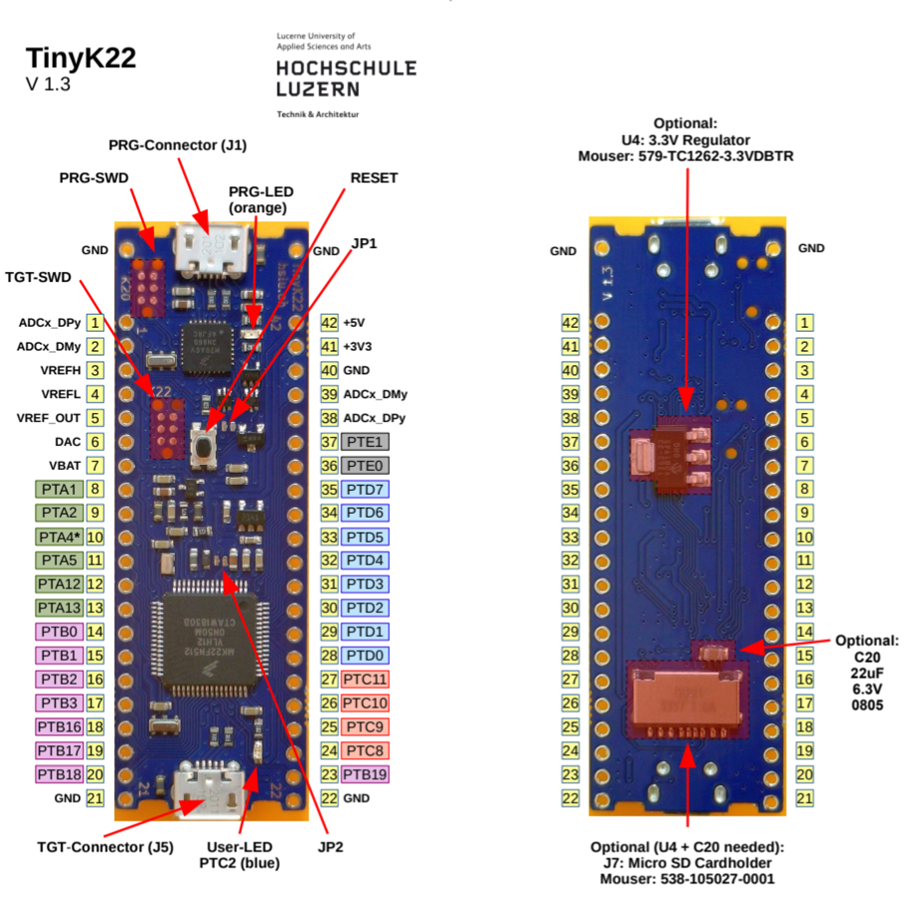
\includegraphics[width=0.8\linewidth]{img/Tiny_K22_PCB.png}
    \caption{Tiny K22. Quelle: \cite{tiny-K22-Pinout}}
    \label{fig:Tiny_K22_PCB}
\end{figure}


Das \gls{tinyk22} \acrshort{pcb} bietet insgesamt 28 Pins (Abb. \ref{fig:Tiny_K22_PCB}). Diese Pins können flexibel als \acrfull{ftm}, \acrfull{adc}, \acrfull{iic}, \acrfull{spi}, \acrshort{uart}, Input- oder Output-Pins konfiguriert werden.

Im Rahmen des Projekts wurden 25 Pins verwendet (Abb. \ref{fig:Tiny_K22_Pinout_definition}). Die zeitkritischen Funktionen werden direkt auf dem \gls{tinyk22} verarbeitet.

\begin{figure}[H]
    \centering
    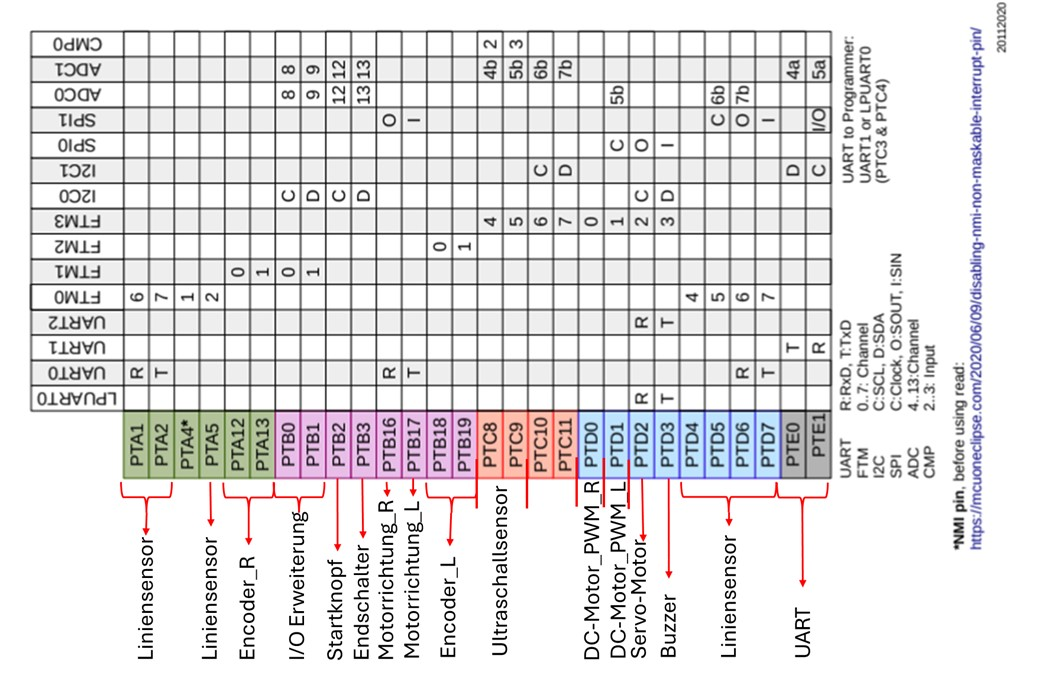
\includegraphics[width=0.8\linewidth, angle=-90]{img/Tiny_K22_Pinout_definition.jpg}
    \caption{Pinout Tiny K22. Quelle: \cite{tiny-K22-Pinout}}
    \label{fig:Tiny_K22_Pinout_definition}
\end{figure}

Folgende Zuweisungen wurden vorgenommen:
\begin{itemize}
    \item Encoder-Auswertung: Der Mikrocontroller nutzt die integrierte Quadratur-Encoder-Auswertung auf Timer 1 und Timer 2.
    \item Linienerfassung: Diese Funktion belegt den gesamten Timer 0.
    \item Motorsteuerung, Ultraschallsensor, Buzzer und Servomotor: Diese teilen sich Timer 3, da keine weiteren Timer zur Verfügung stehen. Dies führt dazu, dass die Motoren im hörbaren Frequenzbereich betrieben werden. Dieser Umstand ist jedoch akzeptabel, da keine Vorgaben zur maximalen Lautstärke existieren.
    \item Zusätzlich wird ein \acrshort{iic}-Bus für zeitunkritische Funktionen verwendet. Zu diesen gehören die Ziellampe und die Zielauswahlschalter.
\end{itemize}

Durch diese Zuweisung wird sichergestellt, dass die zeitkritischen Aufgaben effizient verarbeitet werden, während gleichzeitig Flexibilität für zusätzliche Funktionen über den \acrshort{iic}-Bus gewährleistet bleibt.


\subsubsection*{Liniensensor}
\addcontentsline{toc}{subsubsection}{Liniensensor}


Der Liniensensor wird als Array verwendet, das heisst, es werden Sensoren nebeneinander auf dem \acrshort{pcb} angeordnet. Die Sensoren sind Phototransistoren die lichtabhängig sind. Das Array ist dafür da die Linie zu erfassen und allfällige Korrekturen einzuleiten. Damit man den Wegpunkt erkennen kann werden vor und nach dem Array je ein Sensor verbaut. Es sind 7 Pins auf dem \gls{tinyk22} reserviert (Abb. \ref{fig:Tiny_K22_Pinout_definition}) für den Liniensensor. Die 7 Pins werden die einzelnen Sensoren auslesen und die Werte verarbeiten. Mithilfe von Kondensatoren werden die Entladezeiten für die Auswertung genutzt (Abb. \ref{fig:Liniensensor_Schaltung}). Mit der Timerfunktion \verb|Input Capture| kann die fallende Flanke, die bei der Entladung auftritt, detektiert werden. \verb|Input Capture| gibt die Zeit zurück von dem Zeitpunkt, bei dem der Kondensator sich anfängt zu entladen, bis zu dem Zeitpunkt, bei welchem die Spannung 0V ist.

\begin{figure}[H]
    \centering
    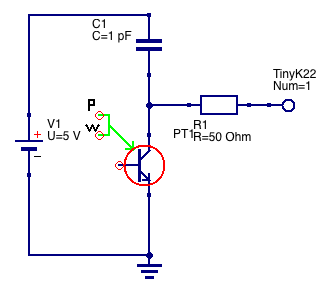
\includegraphics[width=0.4\linewidth]{img/Liniensensor_Schaltung.png}
    \caption{Schaltungsprinzip Liniensensor}
    \label{fig:Liniensensor_Schaltung}
\end{figure}

\subsubsection*{Ultraschall}
\addcontentsline{toc}{subsubsection}{Ultraschall}

Es ist noetig, dass der Roboter weiss, wenn er sich vor einem Hindernis befindet. Dafuer soll ein Arduino Ultraschallsensor verwendet werden. Der Abstand wird gemessen, indem Ultraschallwellen ausgesendet werden und ausgewertet wird, wie lange es dauerte bis die Wellen wieder zurück empfangenen werden. Daraus kann die Distanz berechnet werden.

Mit dem Arduino Ultraschall wurden Tests durchgefuehrt. Dazu wurde ein kurzes Skript geschrieben, um die Messungen der Arduinos auszulesen (https://gist.github.com/dimschlukas/cf343803080f90a1756911548723bcb1). Der Arduino wurde auf einem Tisch platziert und die Hindernisse wurden davorgehalten und langsam auf den Sensor zu bewegt. So konnte beobachtet werden, wie der Sensor bemerkt, dass die Objekte naeher kommen.

Damit Barrieren angehoben werden koennen, muss der Abstand dazu erkannt werden koennen. Dazu wurden Tests durchgefuehrt. Der Ultraschallsensor war in der Lage auf einige Zentimeter genau die Distanz korrekt zu messen.

Ebenfalls soll der Roboter erkennen koennen, wenn er sich vor einer Pylone befindet, damit er nicht in diese reinfaehrt. Dazu wurden ebenfalls Tests durchgefuehrt. Trotz der Kegelform der Pylonen ist es moeglich, die Distanz gut zu messen.

Nun muss der Roboter wissen, vor welchem Hindernis er sich befindet, da die naechsten Schritte des Roboters unterschiedlich sind, je nach Hindernis. Es wurden zwei Moeglichkeiten untersucht, um diese Unterscheidung durchzufuehren:

\begin{itemize}
    \item Zwei Sensoren werden am Roboter angebracht: Der eine davon ist hoeher als die Barriere, damit dieser Barrieren nicht erkennt.
    \item Bei Erkennung eines unerwarteten Hindernisses wird ein Foto gemacht und das Hindernis wird mit Bilderkennung erkannt.
\end{itemize}

Die erste Methode wuerde zwei Ultraschallsensoren benoetigen, die auf unterschiedlichen Hoehen angebracht waeren. Wenn beide ein Objekt vor sich erkennen handelt es sich um eine Pylone, erkennt nur der untere ein Objekt, ist es eine Barriere. Diese Methode wuerde funktionieren, wie aus den vorhin erwaehnten Ultraschalltests erkannt wurde.

Die zweite Methode verwendet die selbe Kamera und die selbe Art Objekte auf Bildern zu erkennen, wie in Kapitel \ref{subsubsection:bilderkennung} beschrieben. Dies wuerde ebenfalls funktionieren. Die Tests zu der Bilderkennung sind im Kapitel \nameref{bilderkennung-protoype} zu finden.

In der folgenden Tabelle sind Vor- und Nachteile beider Methoden aufgelistet.



\begin{table}[H]
\centering
\small
\begin{tabularx}{\textwidth}{|X|X|}
        \hline
        \textbf{2 Sensoren} & \textbf{Kamera und Bilderkennung}\\
        \hline
        + Weniger Rechenpower noetig. & + Keine zusaetzliche Hardware noetig.  \\ \hline
        + Erkennung und Unterscheidung der Hinderniss wird auf einem Rechner durchgefuehrt.  & + Navigation berechnet naechste Schritte und liest ebenfalls die Hindernisart aus.  \\ \hline
        + Simpel. & Buchstabe C erkennen\\ \hline 
        EasyOCR & Buchstabe A erkennen\\ \hline
        EasyOCR & Buchstabe B erkennen  \\ \hline
        EasyOCR & Buchstabe C erkennen & C wird erkannt \\ \hline
        ORB & Buchstabe A erkennen & A wird erkannt \\ \hline
        ORB & Buchstabe B erkennen & B wird erkannt \\ \hline

\end{tabularx}
    \caption{Hindernisse erkennen: 2 Methoden}
\label{tab:obstacle-sensor}
\end{table}


Aus der Tabelle geht hervor, dass es mehr Vorteile fuer die Methode mit der Kamera gibt. Diese wird in PREN 2 vertieft erarbeitet werden.

\subsubsection*{Servomotor}
\addcontentsline{toc}{subsubsection}{Servomotor}


Der Servomotor wurde direkt am Greifer Prototyp getestet. In der folgenden Tabelle \ref{tab:testpunkte Servomotor} sind die Messergebnisse eingetragen, welche positiv ausgefallen sind. Der Servomotor wurde bei zwei unterschiedlichen Frequenzen getestet. Dabei war die Betriebsspannung immer auf 5V. Es soll getestet werden, ob der Greifer das Hindernis auf die geforderten 7.5mm anheben kann. Das \acrshort{pwm} Signal wurde mit einem Tektronix AFG1022 generiert, bei welchem der \gls{duty-cycle} mit einem Drehregler verstellt werden kann.

\begin{table}[H]
\centering
\small
\begin{tabularx}{\textwidth}{|c|X|X|X|l|}
        \hline
        \textbf{Index} & \textbf{Kurzbeschreibung} & \textbf{Kriterium zur Erfüllung} & \textbf{Messergebnisse} & \textbf{Bemerkungen} \\
        \hline
        1 & PWM mit 10kHz & Motor soll drehen & Der Motor dreht nicht & Test nicht erfüllt \\ \hline
        2 & PWM mit 400Hz & Motor soll drehen & Bei 15\% Duty Cycle dreht Servomotor 180 Grad & Test erfüllt \\ \hline
        3 & Betriebsspannung mit 5V & Betrieb damit \acrshort{pwm} funktioniert  & PWM funktioniert & Test erfüllt\\ \hline
        4 & Motor drehen bis Hindernis angehoben & Hindernis wird angehoben & Greifer hebt Hindernis 7.5mm hoch, bei 32\% Duty Cylce & Test erfüllt \\ \hline
\end{tabularx}
    \caption{Testergebnisse des Servomotors am Greifer.}
\label{tab:testpunkte Servomotor}
\end{table}

\newpage

Der Startpunkt des Tests wurde bei einem \gls{duty-cycle} von 86\% festgelegt. Wie in der Abbildung \ref{fig: Greiferposition offen: Duty Cycle 86} ersichtlich wird, war das die Position, bei welcher der Greifer offen ist.

\begin{figure}[H]
    \centering
    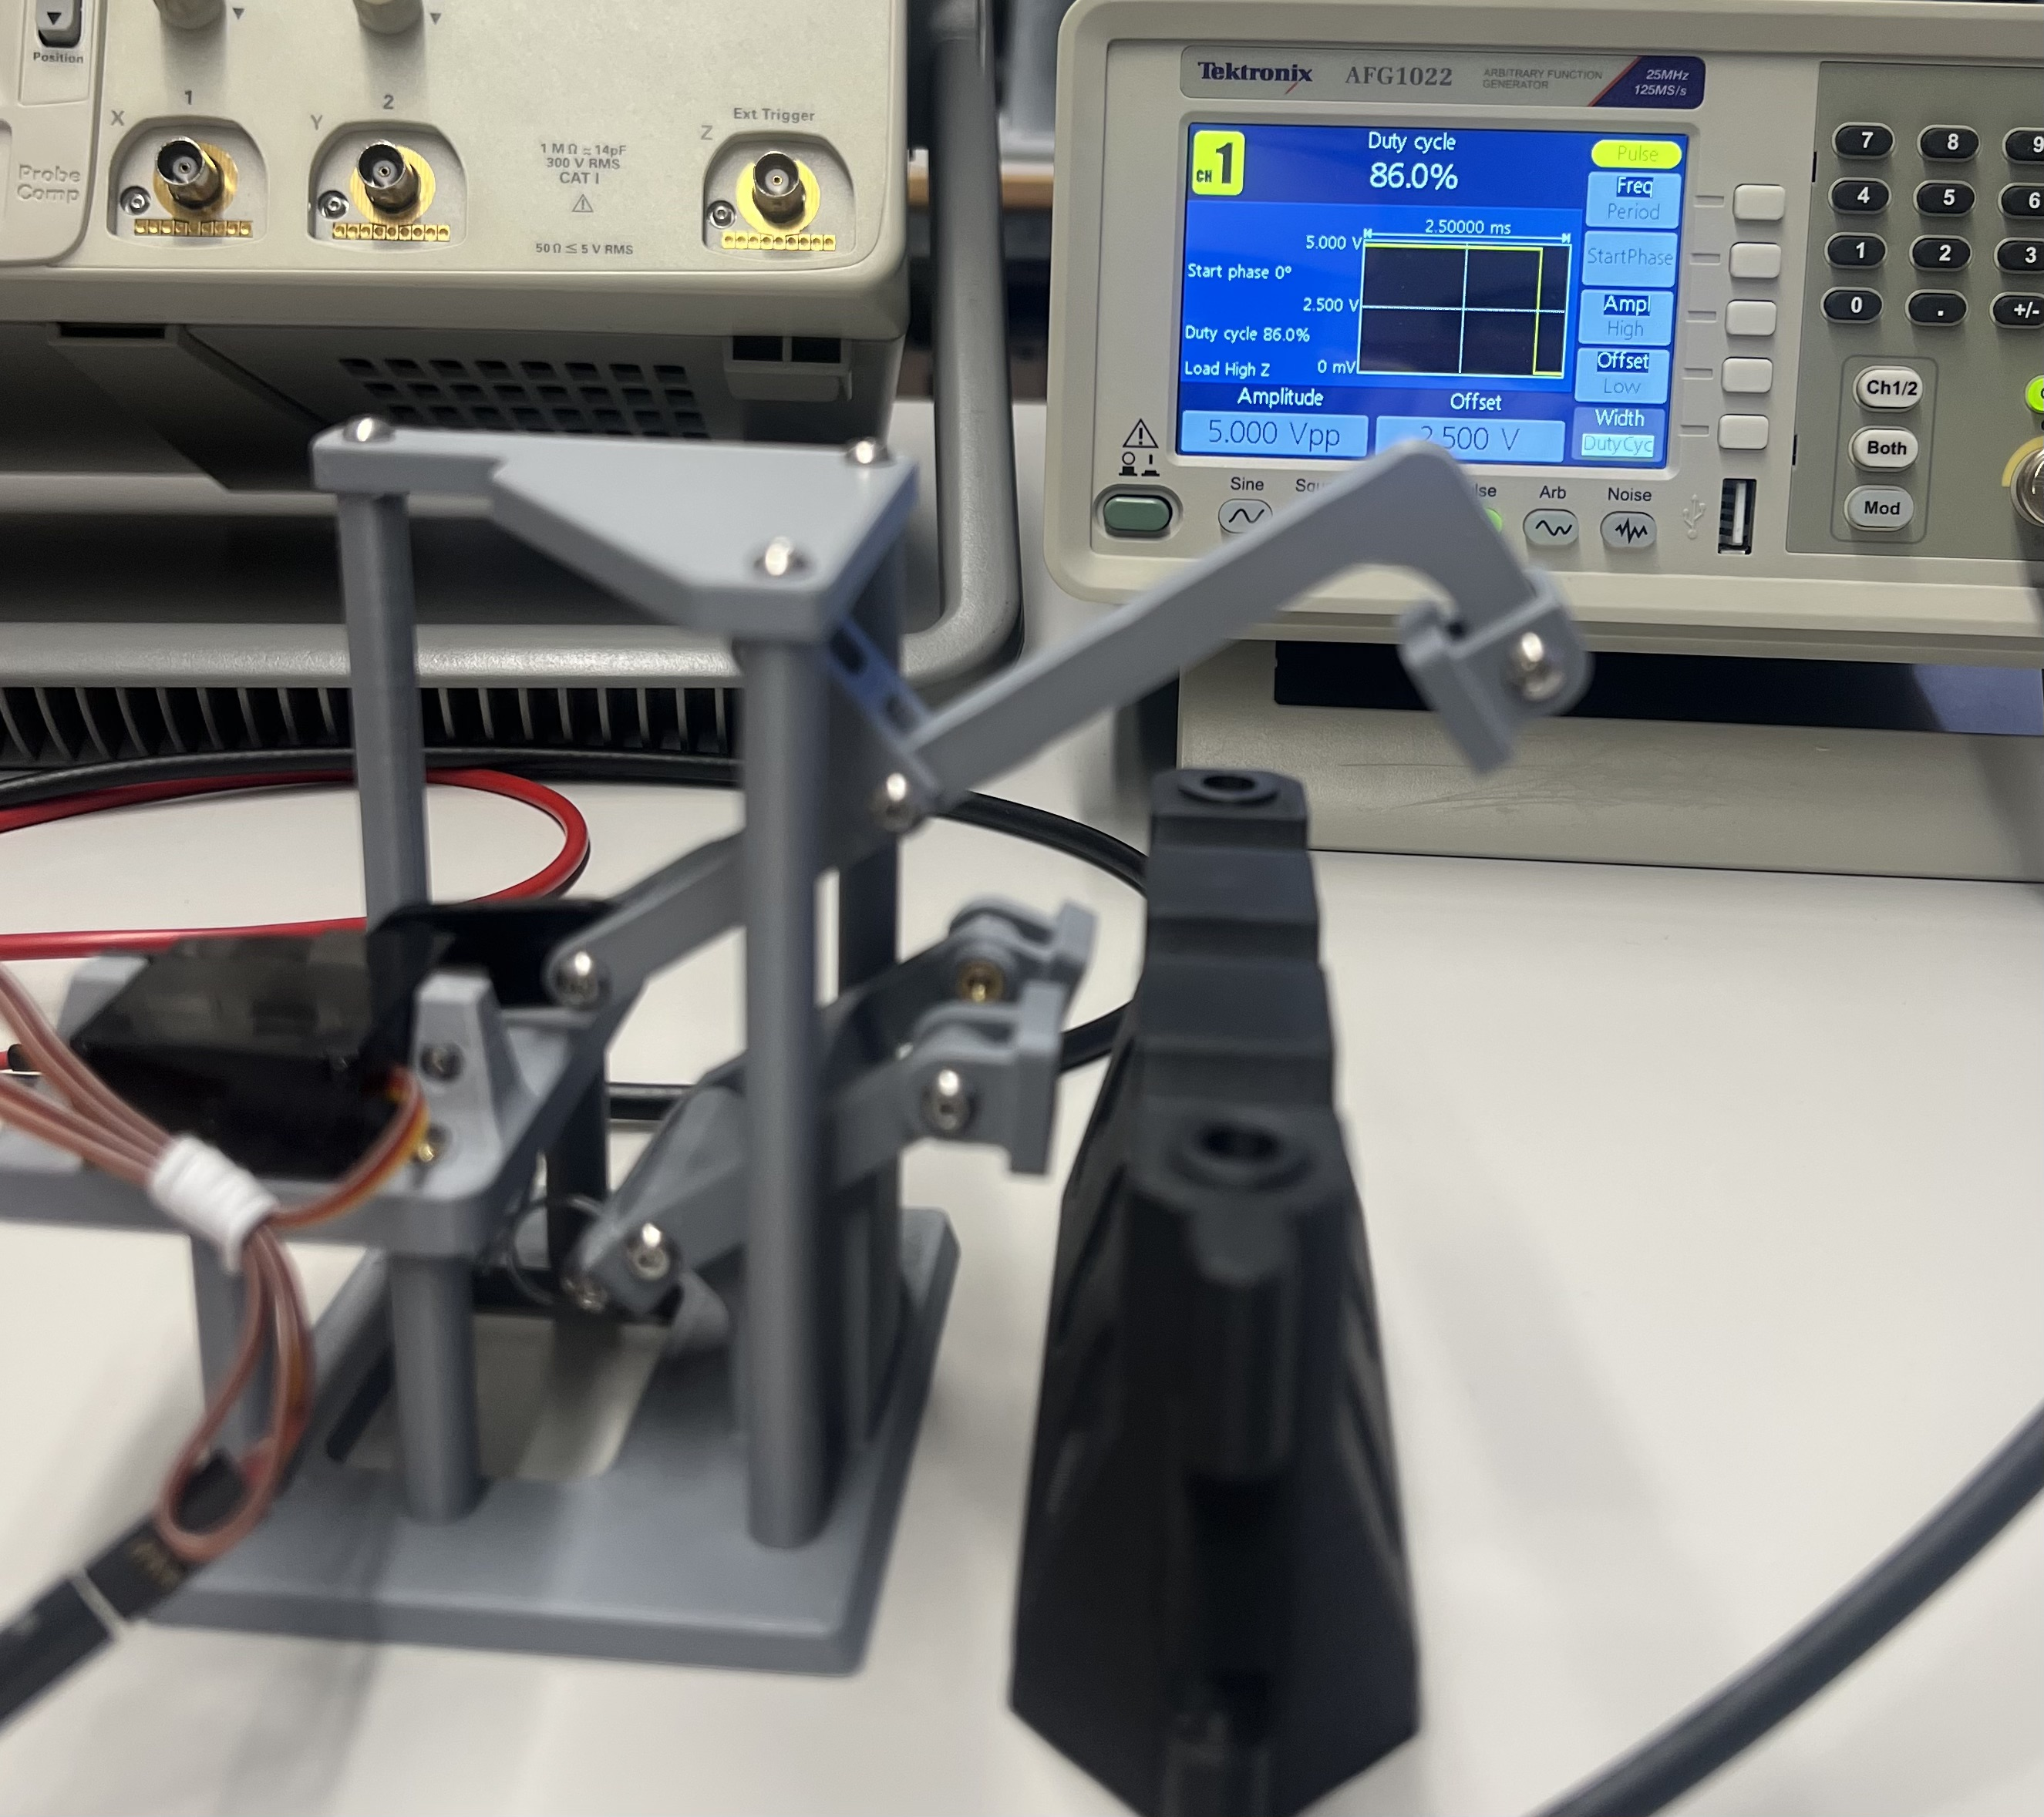
\includegraphics[width=0.8\linewidth]{img/ServoGreifferoffen.jpeg}
    \caption{Greiferposition offen: Duty Cycle 86\%}
    \label{fig: Greiferposition offen: Duty Cycle 86}
\end{figure}

\newpage

Der nächste Messpunkt ist nachdem der \gls{duty-cycle} so minimiert wurde, bis der Greifer das Hindernis klemmt aber noch nicht angehoben hat. Dies ist ersichtlich in Abbildung \ref{fig: Greiferposition eingeklemmt: Duty Cycle 47}.

\begin{figure}[H]
    \centering
    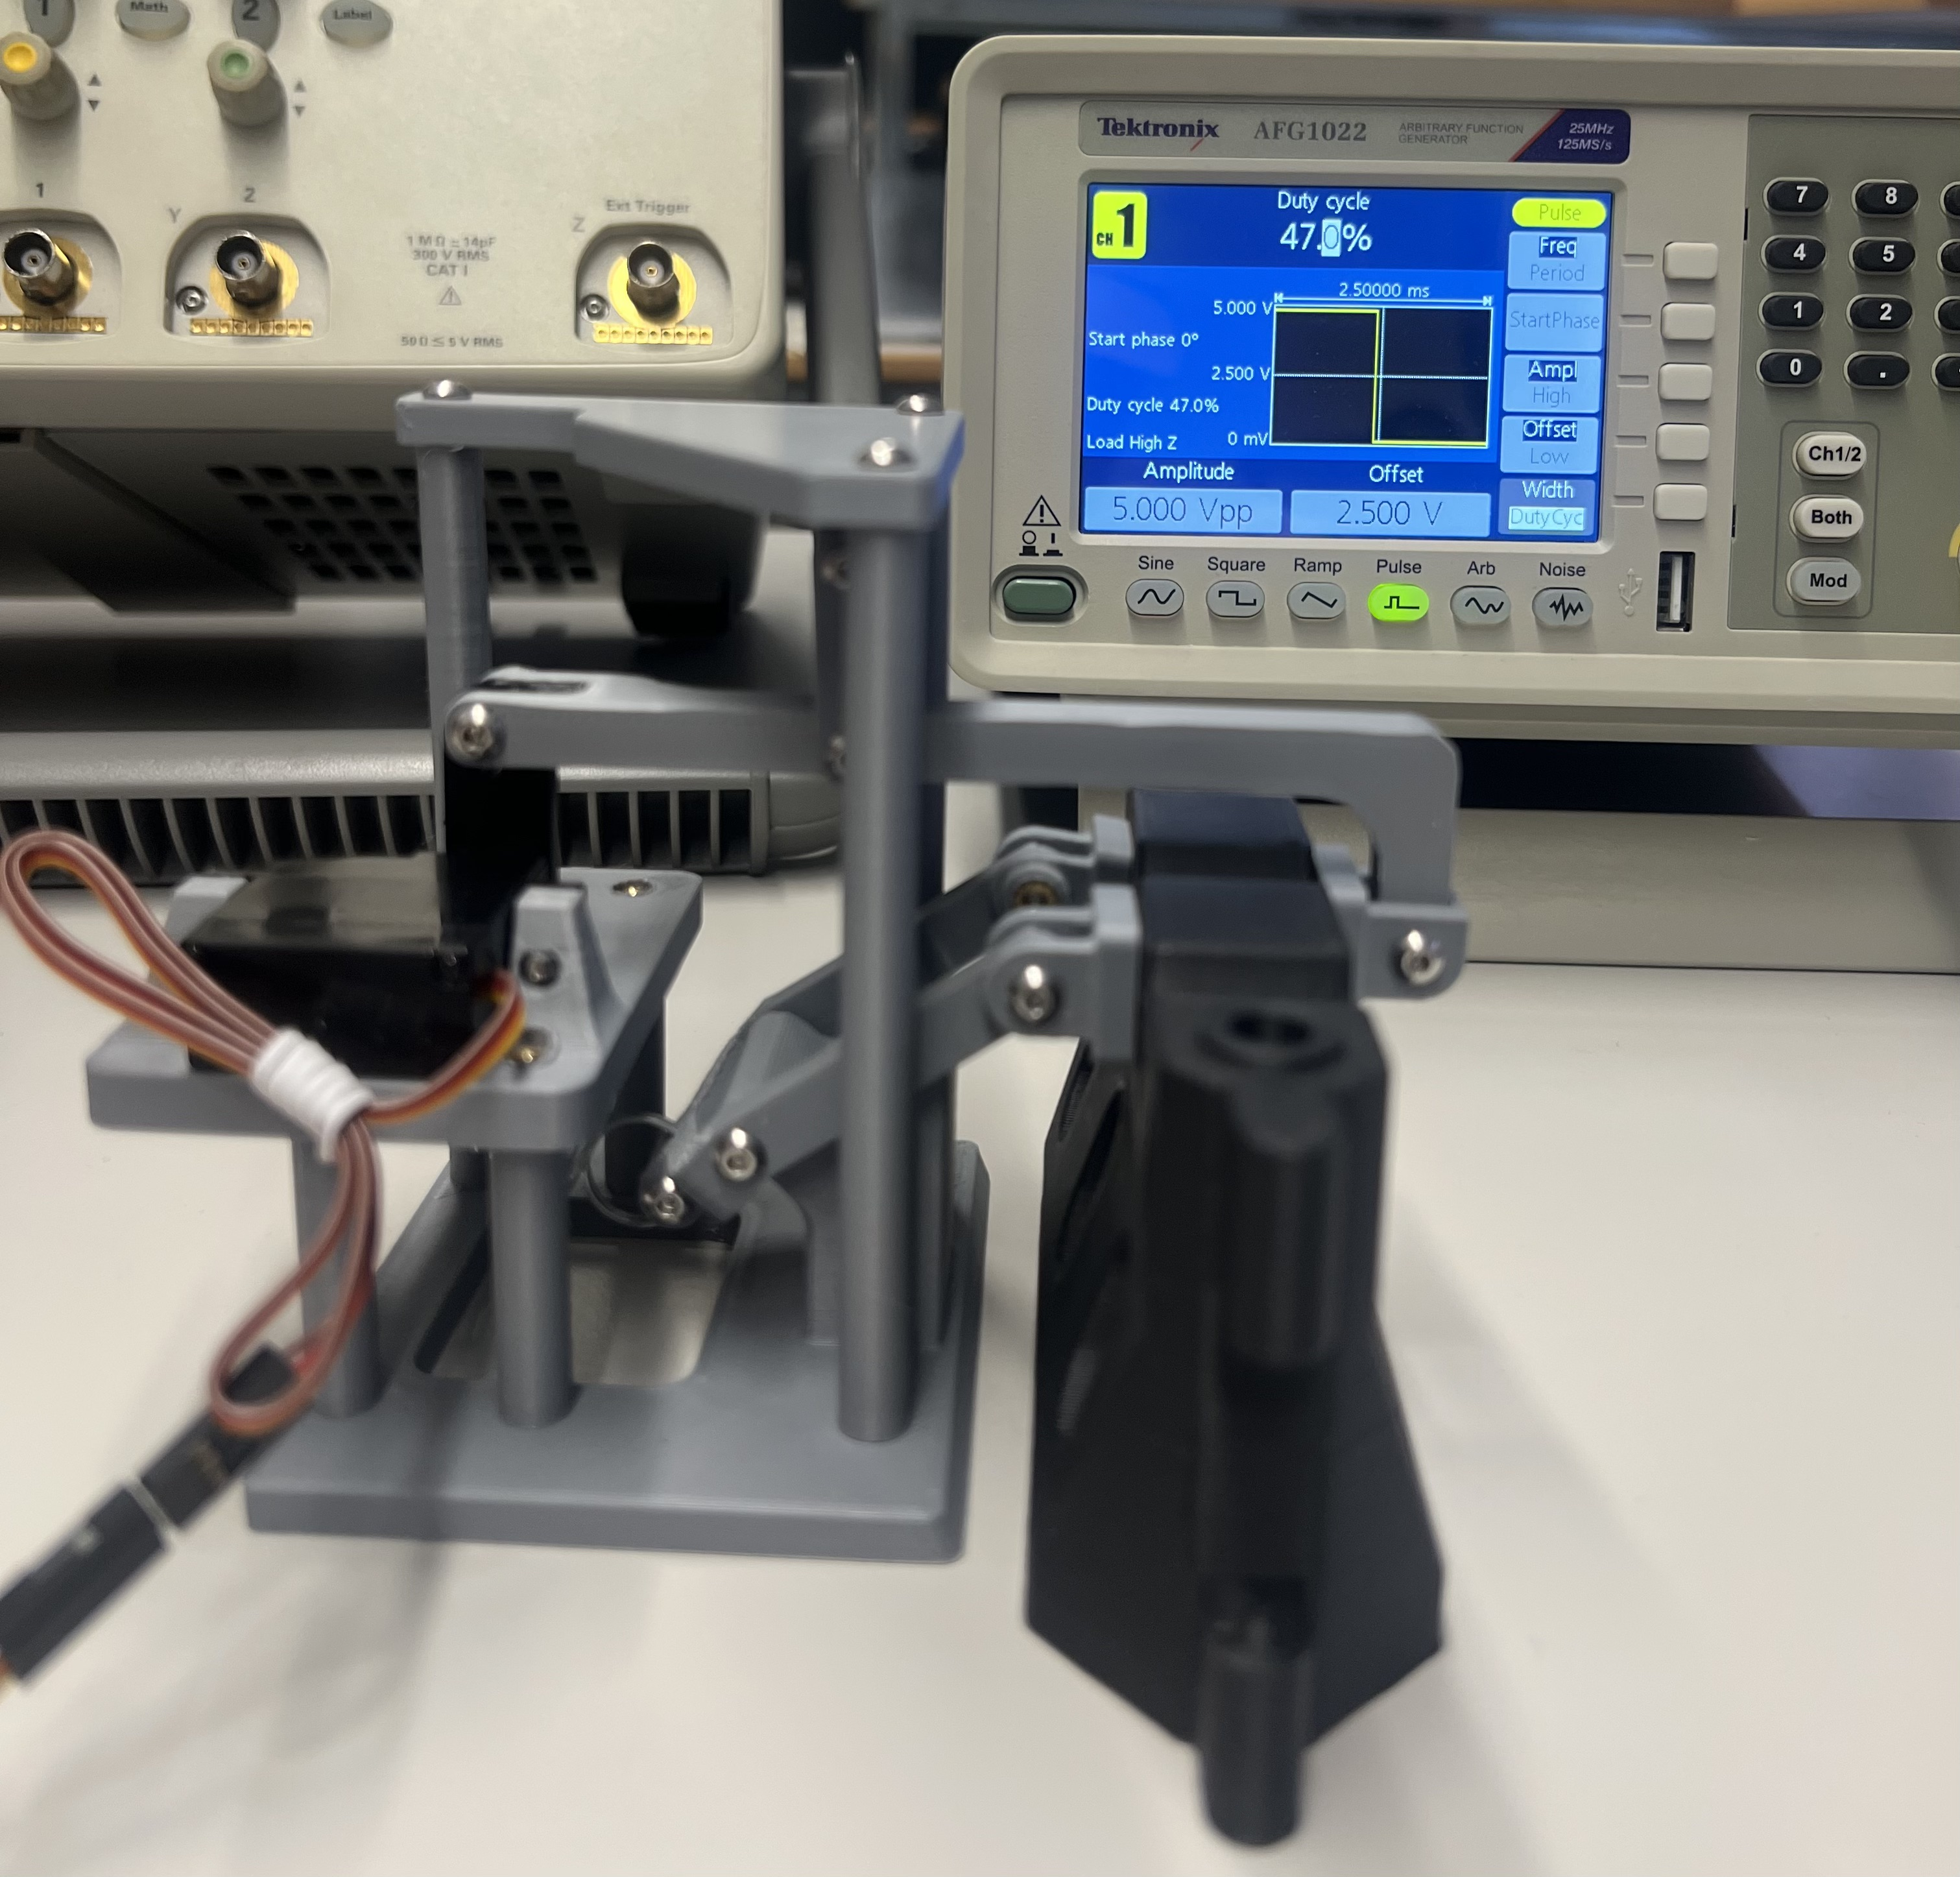
\includegraphics[width=0.8\linewidth]{img/ServoGreiferKlemmt.jpeg}
    \caption{Greiferposition eingeklemmt: Duty Cycle 47\%}
    \label{fig: Greiferposition eingeklemmt: Duty Cycle 47}
\end{figure}

\newpage

Damit die Anforderung von Tabelle \ref{tab:test-gripper-prototype-1} mit der Hubhöhe erfüllt wird, musste der \gls{duty-cycle} auf 32\% reduziert werden. Somit ist auf der Abbildung \ref{fig: Greiferposition angehoben: Duty Cycle 32} das um 7.5mm angehobene Hindernis zu sehen.

\begin{figure}[H]
    \centering
    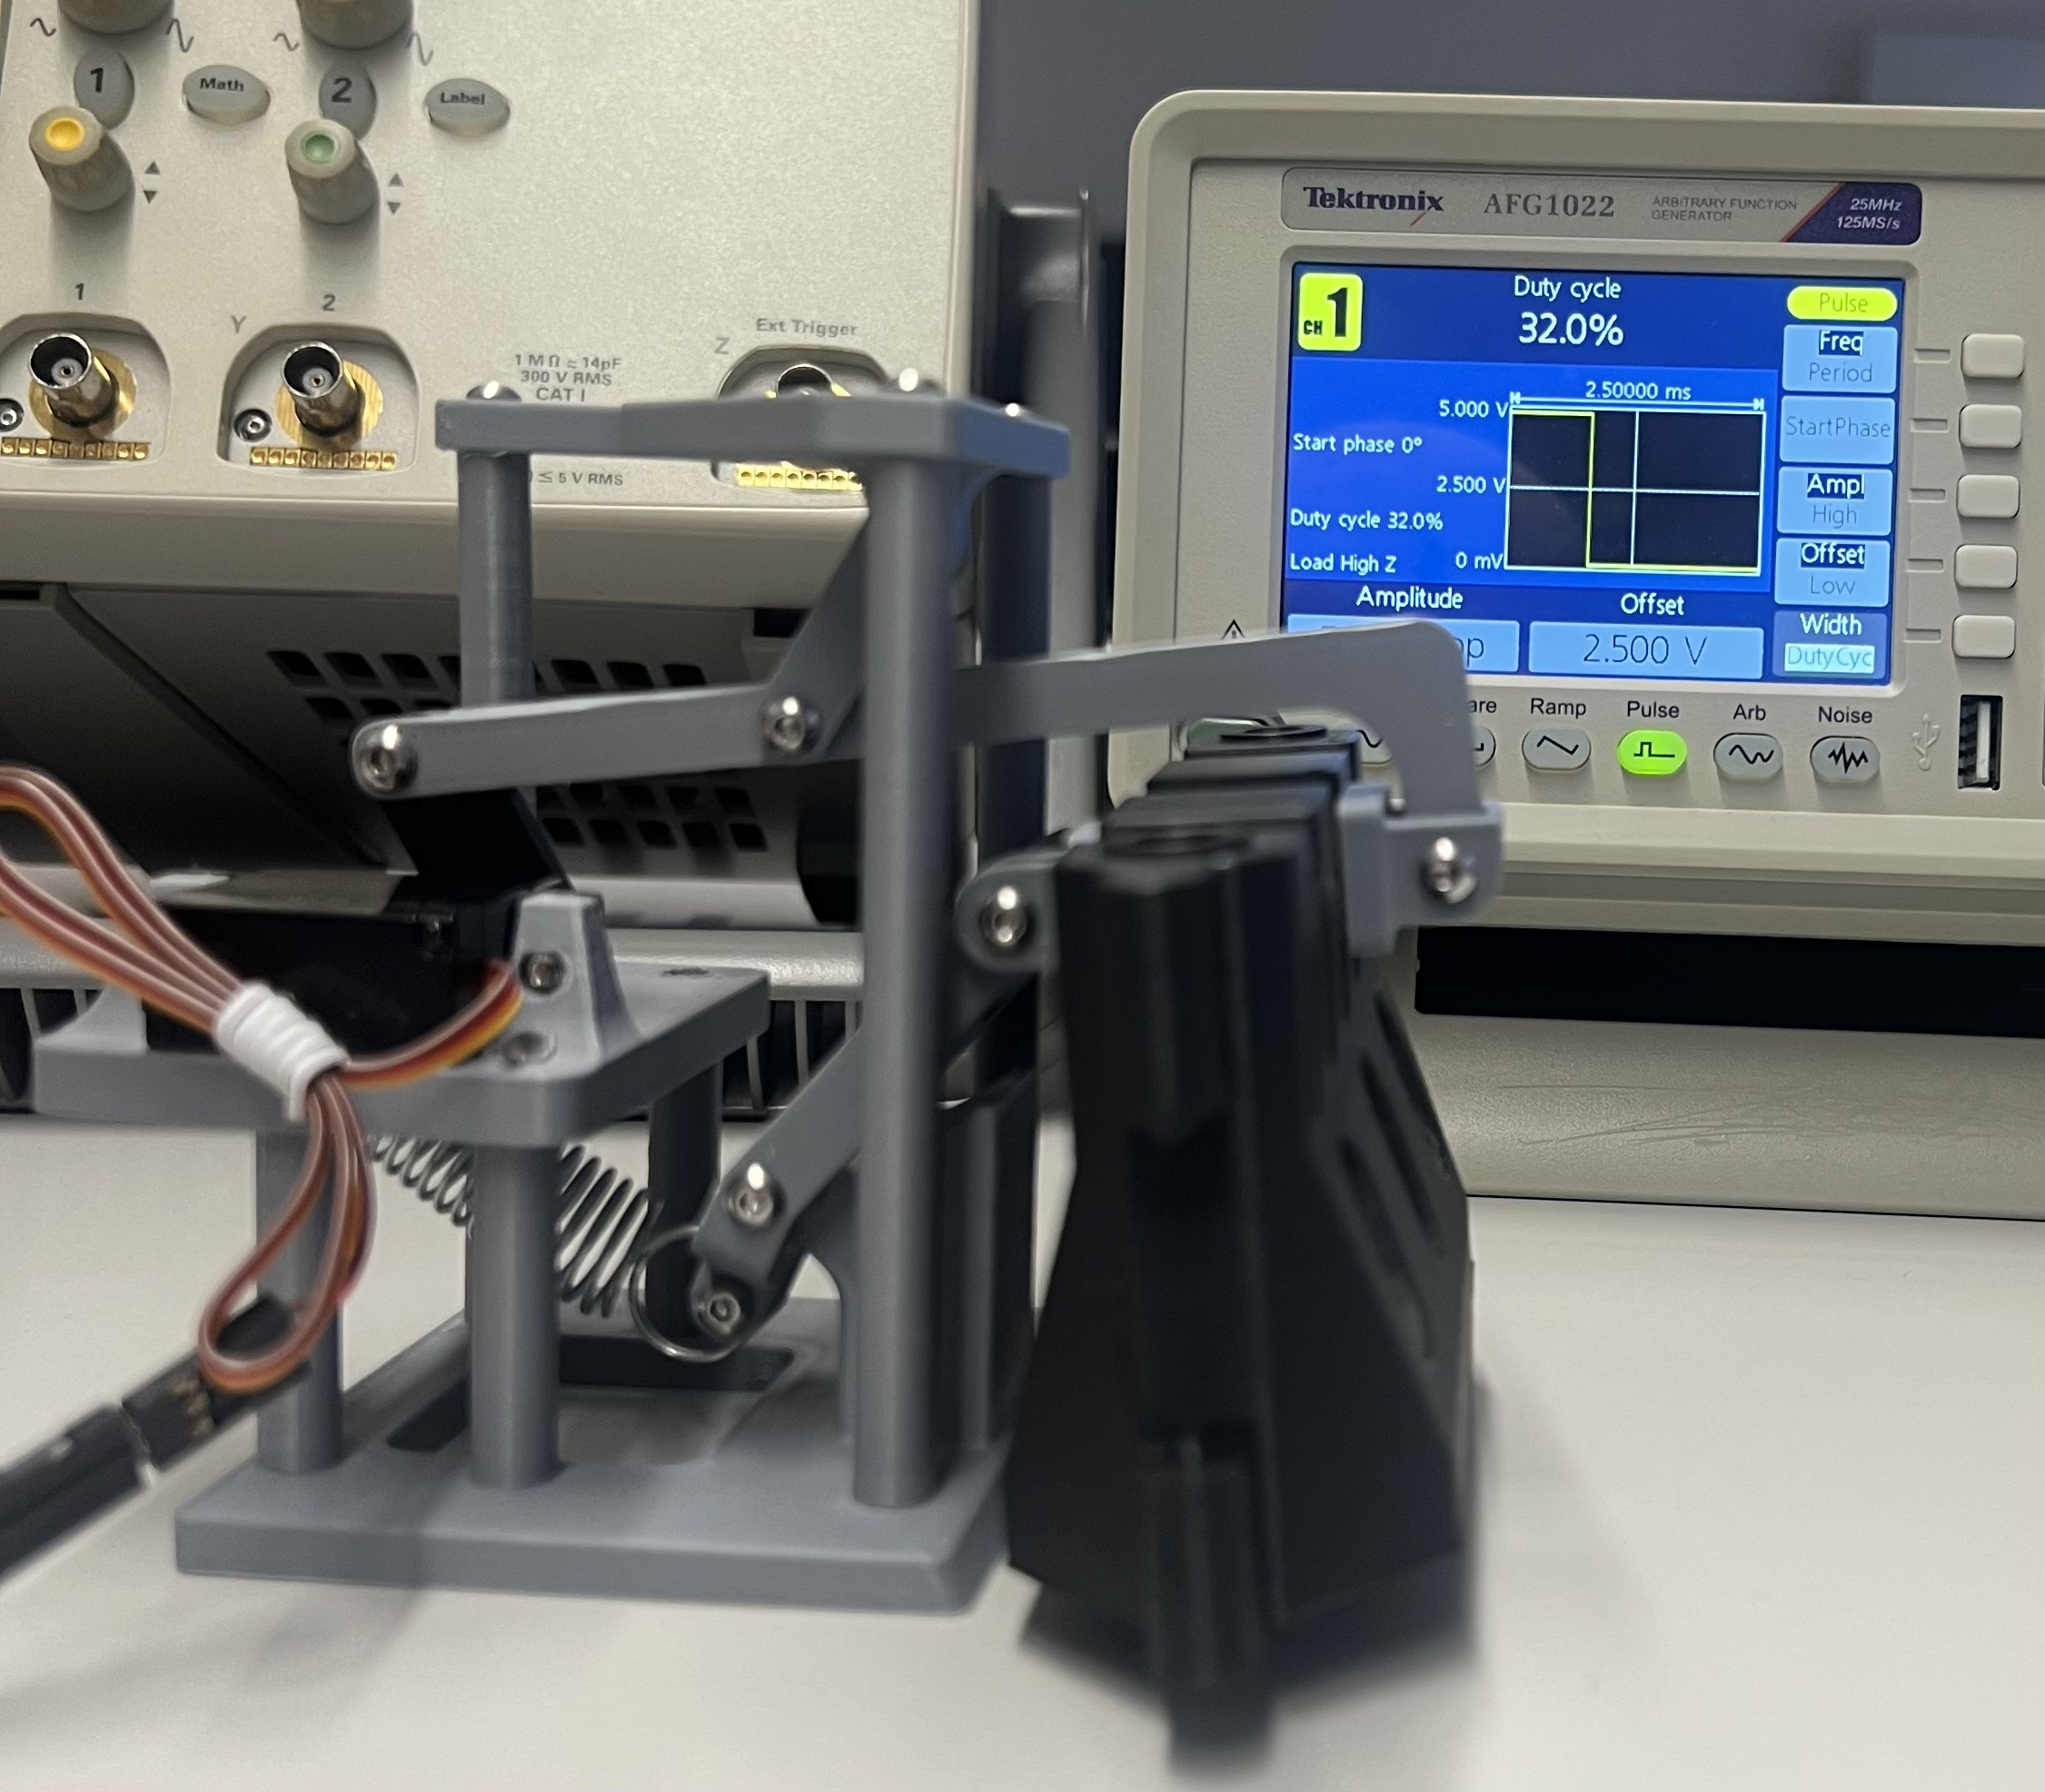
\includegraphics[width=0.8\linewidth]{img/ServoHindernisAngehoben.jpeg}
    \caption{Greiferposition eingeklemmt: Duty Cycle 32\%}
    \label{fig: Greiferposition angehoben: Duty Cycle 32}
\end{figure}